\documentclass[12pt]{elsarticle}

\usepackage[utf8]{inputenc}
\usepackage[T1]{fontenc}
\usepackage{amsmath,amsfonts,amssymb,amsthm}
\usepackage{newtxtext}
\usepackage{newtxmath}
\usepackage{graphicx}
\usepackage{algorithm}
\usepackage{algorithmic}
\usepackage[hidelinks]{hyperref}
\pdfstringdefDisableCommands{\let\corref\relax\let\cnotenum\relax\let\cortext\relax}
\usepackage{xcolor}
\usepackage{subcaption}
\usepackage{booktabs}
\usepackage{mathtools}
\usepackage{float}
\usepackage{tikz}
\usepackage{placeins}


\usetikzlibrary{arrows.meta, positioning}

\newtheorem{theorem}{Theorem}
\newtheorem{lemma}{Lemma}
\newtheorem{corollary}{Corollary}
\newtheorem{proposition}{Proposition}
\newtheorem{definition}{Definition}
\theoremstyle{remark}
\newtheorem{remark}{Remark}
\newtheorem{assumption}{Assumption}

\setlength{\textfloatsep}{8pt plus 2pt minus 2pt}
\setlength{\floatsep}{8pt plus 2pt minus 2pt}
\setlength{\intextsep}{8pt plus 2pt minus 2pt}
\setlength{\abovecaptionskip}{4pt}
\setlength{\belowcaptionskip}{2pt}

\renewcommand{\topfraction}{0.9}
\renewcommand{\bottomfraction}{0.9}
\renewcommand{\textfraction}{0.05}
\renewcommand{\floatpagefraction}{0.92}

\DeclareMathOperator{\diag}{diag}
\DeclareMathOperator{\col}{col}
\DeclareMathOperator{\row}{row}
\DeclareMathOperator{\rank}{rank}
\DeclareMathOperator{\vecs}{vecs}
\DeclareMathOperator{\trace}{tr}
\newcommand{\R}{\mathbb{R}}
\newcommand{\N}{\mathbb{N}}
\newcommand{\C}{\mathbb{C}}
\newcommand{\ones}{\mathbb{1}}
\newcommand{\bx}{\boldsymbol{x}}
\newcommand{\bu}{\boldsymbol{u}}
\newcommand{\be}{\boldsymbol{e}}

\journal{IFAC Journal of Systems and Control}

\linespread{1.0}\selectfont
\emergencystretch=1em
\hbadness=10000
\vbadness=10000

\begin{document}

\begin{frontmatter}

\title{Data-Driven Q-Learning for Consensus and Multi-Consensus Control of Discrete-Time Linear Multi-Agent Systems}

\author[ttu]{Md Nur-A-Adam Dony}
\ead{mdony42@tntech.edu}

\author[ttu]{Syed Ali Asad Rizvi\corref{cor1}}
\ead{srizvi@tntech.edu}
\cortext[cor1]{Corresponding author.}

\affiliation[ttu]{organization={Department of Electrical and Computer Engineering, Tennessee Technological University},
            city={Cookeville},
            postcode={38505},
            state={TN},
            country={USA}}

\begin{abstract}
This paper presents data-driven Q-learning algorithms for consensus and multi-consensus control of discrete-time linear multi-agent systems. Both state feedback and output feedback formulations learn the gains of a predictor-based consensus protocol directly from measured data, without knowledge of the agent dynamics. The state feedback algorithm recovers both gains from a single agent's state-input trajectory, with convergence to the discrete algebraic Riccati equation solution established rigorously. The output feedback extension learns the input-coupling gain and reconstructs the inter-agent disagreement feedback from input-output data alone, eliminating full state measurement while preserving the consensus properties of the underlying design. A numerical robustness analysis demonstrates the advantage of the data-driven gains under parametric model uncertainty, and simulations on multi-consensus, formation control, and vehicle-platoon scenarios validate the results against the model-based benchmark.
\end{abstract}

\begin{keyword}
Multi-agent systems \sep Consensus control \sep Q-learning \sep Output feedback \sep Data-driven control \sep Discrete-time systems
\end{keyword}

\end{frontmatter}

%% ===================================================================
\section{Introduction}
\label{sec:intro}
%% ===================================================================

Consensus control of networked multi-agent systems (MAS) is a fundamental problem in distributed control theory, with applications in formation control of unmanned vehicles~\cite{francis2016,dony2021distributed,dong2020tracking}, synchronization of complex networks~\cite{dorfler2014,li2010}, distributed filtering~\cite{battistelli2014}, and opinion dynamics in social networks~\cite{proskurnikov2017}. The central objective is to design distributed control laws that drive all agents toward common trajectories using only local information exchanged over a communication graph.

A well-known challenge distinguishes the discrete-time and continuous-time settings. For continuous-time MAS, arbitrarily fast convergence to consensus can be achieved simply by increasing the scalar coupling gain~\cite{li2014,liu2021}. In sharp contrast, for discrete-time systems, the coupling gain is constrained to be small---typically inversely proportional to the largest eigenvalue of the Laplacian matrix---to maintain closed-loop stability~\cite{ma2015,ren2010,xiao2004}. This constraint fundamentally limits the achievable convergence rate.

Recently, Cacace et al.~\cite{cacace2024} proposed a predictor-based consensus protocol for discrete-time LTI MAS that overcomes this limitation through an implicit feedback law involving both the state and input of neighboring agents, recovering arbitrary convergence rate via multiple consensus steps per sampling period. The analysis extends to weakly connected digraphs through almost equitable partitions~\cite{monaco2019}, and the design requires solving a single DARE for two gain matrices $F$ and $G$. However, this requires exact knowledge of $(A,B)$, which may not be available in practice due to modeling errors, parametric variations, or discretization approximations~\cite{dony2020tracking,dong2020tracking,dony2021robust}.

Reinforcement learning (RL) offers a model-free alternative~\cite{lewis2009}. Q-learning solves the LQR problem without system knowledge~\cite{bradtke1994} using policy iteration (PI) or value iteration (VI), and output feedback RL reconstructs the state from input-output data~\cite{lewis2009,rizvi2022}. For MAS, Zhang et al.~\cite{zhang2011} developed RL-based optimal synchronization, and related data-driven methods include safe RL for discrete event systems~\cite{dony2025debf}, battery balancing~\cite{dony2026battery}, and Koopman-based control~\cite{dony2024koopman}. However, these methods address the standard explicit protocol $u_i = -\kappa \sum_j F(x_i - x_j)$. The predictor-based protocol of~\cite{cacace2024} has a fundamentally different implicit structure: $u_i$ depends on both states \emph{and inputs} of neighbors through $G$, requiring a matrix inversion $(I + \bar{\mathcal{L}} \otimes G)^{-1}$ to resolve the coupling, which prevents direct application of existing RL-based MAS methods. Integrating model-free RL with predictor-based consensus protocols has not been addressed.

\begin{itemize}
\item Novelty and context: In this paper, we learn the consensus gains of the predictor protocol of~\cite{cacace2024} directly from data. The entry point is structural: the consensus DARE coincides with the LQR Riccati equation for $R = I_m$, so single-agent Q-learning can extract both gains $F$ and $G$ without knowledge of $(A,B)$. This equivalence is not itself the contribution; a direct composition of established Q-learning~\cite{bradtke1994,lewis2009,rizvi2022} with the protocol fails on three counts that the paper resolves: (a)~the protocol is implicit in $u_i$ through $G(u_i-u_j)$, which blocks existing RL-based MAS methods~\cite{zhang2011} and forces a graph-independent single-agent formulation; (b)~output-feedback Q-learning returns the absolute regulator $-K^*x_i$, which drives each agent to the origin, so consensus instead requires reconstructing the inter-agent disagreement $F(x_i-x_j)$ from input-output data (Proposition~\ref{prop:disagreement}); and (c)~only \emph{exact} recovery of the DARE solution preserves the arbitrary convergence rate of~\cite{cacace2024}. The novelty therefore lies in the linkage between two established but previously unconnected areas---data-driven LQR reinforcement learning and predictor-based discrete-time consensus---and in the new capability this linkage enables. Table~\ref{tab:comparison} summarizes these distinctions.
\item Impact and insight: The resulting framework removes the model requirement from a consensus design whose principal appeal is its arbitrary convergence rate, extending its applicability to systems with uncertain, drifting, or poorly discretized dynamics. The insight that both predictor gains reside in the LQR Q-function---with $G$ obtained from the input block that the absolute regulator discards---and that inter-agent disagreement feedback can be reconstructed purely from input-output filter states, is transferable to other implicit or input-coupled distributed control structures.
\end{itemize}

The specific contributions are:
\begin{enumerate}
    \item[(i)] A single-agent learning architecture that decouples the computation of $(F,G)$ from the network topology, since these gains depend only on $(A,B,Q)$; the learning cost is thus independent of the number of agents.
    \item[(ii)] An output feedback extension that learns the input-coupling gain $G$ and reconstructs the disagreement feedback $F(x_i-x_j)$ from input-output data alone (Proposition~\ref{prop:disagreement}), with no state observer or system identification.
    \item[(iii)] Rigorous convergence proofs showing the Q-learned gains satisfy the DARE and inherit all consensus and multi-consensus guarantees, including arbitrary convergence rate.
    \item[(iv)] Quantitative robustness analysis demonstrating that Q-learned gains maintain superior stability margins and lower control costs compared to model-based gains under parametric uncertainty.
    \item[(v)] Comprehensive simulation validation on multi-consensus, formation control, and vehicle-platoon scenarios, benchmarked against the model-based design of~\cite{cacace2024}.
\end{enumerate}

The paper follows the journal structure. Section~\ref{sec:methods} (Methods) presents the preliminaries, the problem formulation, and the state feedback and output feedback Q-learning algorithms with their convergence guarantees. Section~\ref{sec:results} (Results) reports the simulation studies. Section~\ref{sec:discussion} (Discussion) analyzes computational complexity, scalability, communication requirements, robustness, and limitations. Section~\ref{sec:conc} concludes.

\begin{table}[htbp]
\centering
\caption{Comparison of the proposed framework with existing methods.}
\label{tab:comparison}
\small
\setlength{\tabcolsep}{4.5pt}
\begin{tabular}{lccccc}
\toprule
Feature & \cite{cacace2024} & \cite{zhang2011} & \cite{bradtke1994} & \cite{rizvi2022} & \textbf{Proposed} \\
\midrule
Model-free & No & Yes & Yes & Yes & \textbf{Yes} \\
Output feedback & No & No & No & Yes & \textbf{Yes} \\
Arbitrary conv.\ rate & Yes & No & N/A & N/A & \textbf{Yes} \\
Single-agent learning & N/A & No & Yes & Yes & \textbf{Yes} \\
Implicit $G(u_i{-}u_j)$ coupling & Yes & No & No & No & \textbf{Yes} \\
Multi-consensus & Yes & No & No & No & \textbf{Yes} \\
\bottomrule
\end{tabular}
\end{table}

%% ===================================================================
\section{Methods}
\label{sec:methods}
%% ===================================================================

This section formulates the model-free consensus gain learning problem and develops the two proposed algorithms. The methodological novelty is twofold: a structural equivalence that lets a \emph{single-agent} LQR Q-function deliver \emph{both} predictor gains $F$ and $G$ (state feedback), and a disagreement-reconstruction result that realizes the predictor protocol from input-output data alone (output feedback). Neither is available from standard LQR Q-learning~\cite{bradtke1994,lewis2009,rizvi2022}, which produces a single absolute regulator gain for an isolated system and is not connected to a consensus protocol.

\begin{table}[htbp]
\centering
\caption{Notation used throughout the paper.}
\label{tab:notation}
\footnotesize
\setlength{\tabcolsep}{4pt}
\begin{tabular}{@{}llll@{}}
\toprule
\textbf{Symbol} & \textbf{Description} & \textbf{Symbol} & \textbf{Description} \\
\midrule
$\R,\C,\N$ & Real, complex, natural numbers & $\vecs(H)$ & Vectorization of symmetric $H$ \\
$\Re(z)$ & Real part of $z \in \C$ & $\mathcal{L},\bar{\mathcal{L}}$ & Laplacian, modified Laplacian \\
$I_n$ & Identity of size $n$ & $\bar{r}$ & $\min_{\lambda \in \sigma(\mathcal{L})\setminus\{0\}} \Re(\lambda)$ \\
$\ones_N$ & All-ones vector of length $N$ & $F,G$ & Consensus gain matrices \\
$\sigma(A)$ & Spectrum of $A$ & $H,\tilde{H}$ & State/output FB Q-matrices \\
$\rho(A)$ & Spectral radius $\max|\sigma(A)|$ & $K,\bar{K}$ & State/output FB policies \\
$A \otimes B$ & Kronecker product & $x^+$ & $x(t{+}1)$, successor \\
$\col_{i}(x_i)$ & $(x_1^\top,\ldots,x_N^\top)^\top$ & & \\
\bottomrule
\end{tabular}
\end{table}

\subsection{Preliminaries and Problem Formulation}
\label{subsec:prelim}

\subsubsection{Graph Theory}
\label{subsec:graphs}

Consider a digraph $\mathcal{G} = (\mathcal{V}, \mathcal{E})$ with $|\mathcal{V}| = N$ nodes. The in-neighbor set of node $i$ is $\mathcal{N}_i = \{j \in \mathcal{V} : (j,i) \in \mathcal{E}\}$ with in-degree $d_i = |\mathcal{N}_i|$. The Laplacian matrix is $\mathcal{L} = \mathcal{D} - \mathcal{A}$, where $\mathcal{D} = \diag(d_1, \ldots, d_N)$ and $\mathcal{A}$ is the adjacency matrix. By construction, $\lambda_1 = 0 \in \sigma(\mathcal{L})$ with eigenvector $\ones_N$. A digraph has \emph{one reach} if it is weakly connected with a set of root nodes from which all others are reachable; in this case $\lambda_1 = 0$ is simple and $\Re(\lambda_k) > 0$ for $k \geq 2$~\cite{caughman2006}. We define
\begin{equation}
\bar{r} = \min_{\lambda \in \sigma(\mathcal{L}) \setminus \{0\}} \Re(\lambda),
\label{eq:rbar}
\end{equation}
which determines the minimum coupling gain needed for consensus. For general weakly connected digraphs with $\mu$ reaches, $\lambda_1 = 0$ has multiplicity $\mu$~\cite{caughman2006}, and the coarsest almost equitable partition (AEP) $\pi^\star$~\cite{monaco2019} induces the block-triangular Laplacian structure
\begin{equation}
\mathcal{L} = \begin{pmatrix} \diag_{k=1}^{\mu}(\mathcal{L}_k) & 0 \\ \row_{k=1}^{\mu}(\mathcal{M}_k) & \mathcal{M} \end{pmatrix},
\label{eq:L_block}
\end{equation}
where each $\mathcal{L}_k$ has a simple zero eigenvalue and $\sigma(\mathcal{M}) \subset \{z \in \C : \Re(z) > 0\}$.

\subsubsection{System Model and Consensus Problem}
\label{subsec:system}

Consider $N$ identical discrete-time LTI agents with dynamics
\begin{align}
x_i(t+1) &= A x_i(t) + B u_i(t), \label{eq:agent_state} \\
y_i(t) &= C x_i(t), \label{eq:agent_output}
\end{align}
where $x_i \in \R^n$, $u_i \in \R^m$, $y_i \in \R^p$, and common matrices $A \in \R^{n \times n}$, $B \in \R^{n \times m}$, $C \in \R^{p \times n}$. The collective dynamics is
\begin{equation}
\bx^+ = (I_N \otimes A)\bx(t) + (I_N \otimes B)\bu(t),
\label{eq:collective}
\end{equation}
where $\bx = \col_{i=1}^N(x_i) \in \R^{nN}$ and $\bu = \col_{i=1}^N(u_i) \in \R^{mN}$.

\begin{assumption}[Controllability]
\label{ass:controllable}
The pair $(A, B)$ is controllable.
\end{assumption}

\begin{assumption}[Observability]
\label{ass:observable}
The pair $(A, C)$ is observable.
\end{assumption}

\begin{assumption}[Graph Connectivity]
\label{ass:graph}
The communication digraph $\mathcal{G}$ is weakly connected.
\end{assumption}

The consensus problem (for $\mu = 1$) requires $x_i(t) \to A^t x_s(0)$ for all $i$. The multi-consensus problem (for general $\mu$) requires agents in each cell of $\pi^\star$ to converge to a common trajectory~\cite{cacace2024}.

\subsubsection{Predictor-Based Consensus Protocol}
\label{subsec:protocol}

The predictor-based consensus protocol from~\cite{cacace2024} for each agent $i$ is
\begin{equation}
u_i = -\kappa_i \sum_{j \in \mathcal{N}_i} \left[ F(x_i - x_j) + G(u_i - u_j) \right],
\label{eq:protocol}
\end{equation}
where $\kappa_i > 0$, $F \in \R^{m \times n}$, and $G \in \R^{m \times m}$. The term ``predictor-based'' refers to the fact that the protocol contains neighboring input differences $u_i - u_j$ in addition to state differences $x_i - x_j$. Since the one-step disagreement evolution satisfies
\begin{equation}
x_i^+ - x_j^+ = A(x_i - x_j) + B(u_i - u_j),
\label{eq:predictor_interp}
\end{equation}
and the consensus gains satisfy $F = B^\top P A$ and $G = B^\top P B$, the disagreement feedback in~\eqref{eq:protocol} can be written as $F(x_i - x_j) + G(u_i - u_j) = B^\top P(x_i^+ - x_j^+)$. That is, the protocol implicitly accounts for the one-step evolution of the disagreement dynamics. This predictor-like input coupling modifies each disagreement mode through the closed-loop matrix~\eqref{eq:spectrum}, which is the mechanism that removes the small-gain restriction of standard discrete-time consensus protocols~\cite{ma2015}. Note that~\eqref{eq:protocol} is implicit: $u_i$ appears on both the left-hand side and inside the summation through $G(u_i - u_j)$. This coupling is resolved globally through the matrix inversion in the centralized form~\eqref{eq:u_central}, and locally through the iterative $\gamma$-step algorithm~\eqref{eq:dist_init}--\eqref{eq:dist_iter}.

With the modified Laplacian $\bar{\mathcal{L}} = \diag(\kappa_1,\ldots,\kappa_N) \mathcal{L}$, the centralized solution is
\begin{equation}
\bu = -(I_{mN} + \bar{\mathcal{L}} \otimes G)^{-1}(\bar{\mathcal{L}} \otimes F)\bx.
\label{eq:u_central}
\end{equation}
The closed-loop dynamics is $\bx^+ = \Theta \bx$, with spectral decomposition \cite[Lemma~3.1]{cacace2024} giving $\sigma(\Theta) = \bigcup_{\bar{\lambda}_k \in \sigma(\bar{\mathcal{L}})} \sigma(\bar{A}_k)$ where
\begin{equation}
\bar{A}_k = A - B\left(\frac{1}{\bar{\lambda}_k}I_m + G\right)^{-1}F.
\label{eq:spectrum}
\end{equation}

For any $Q = Q^\top > 0$, the model-based design of~\cite[Thm.~3.1]{cacace2024} takes $P = P^\top \succ 0$ solving the DARE
\begin{equation}
A^\top P A - P - A^\top PB(I_m + B^\top PB)^{-1}B^\top PA + Q = 0,
\label{eq:dare}
\end{equation}
and sets
\begin{equation}
F = B^\top P A, \quad G = B^\top P B,
\label{eq:FG_dare}
\end{equation}
for which the closed-loop modes $\bar{A}_k$ in~\eqref{eq:spectrum} are Schur stable provided $\kappa_i \bar{r} > 1$ for all $i$.

The convergence rate is regulated by $Q$~\cite[Remark~3.2]{cacace2024}. For practical deployment, a distributed $\gamma$-step algorithm approximates~\eqref{eq:u_central}~\cite{cacace2024}:
\begin{align}
v_i(t,0) &= -\kappa_i(I_m + \kappa_i d_i G)^{-1} \sum_{j \in \mathcal{N}_i} F(x_i - x_j), \label{eq:dist_init} \\
v_i(t,h{+}1) &= v_i(t,0) + \kappa_i(I_m + \kappa_i d_i G)^{-1} \sum_{j \in \mathcal{N}_i} Gv_j(t,h), \label{eq:dist_iter}
\end{align}
for $h = 0, \ldots, \gamma-1$, with $u_i(t) = v_i(t,\gamma)$.

\textbf{Problem Statement.} The DARE~\eqref{eq:dare} and the gain formulas~\eqref{eq:FG_dare} require explicit knowledge of $(A,B)$, which motivates the following data-driven formulation.

\smallskip
\noindent\textbf{Problem 1} (Model-free consensus gain learning)\textbf{.}
\emph{Given} a performance weight $Q = Q^\top \succ 0$ and measured trajectories
\begin{equation}
\mathcal{D} = \big\{(x_k, u_k)\big\}_{k=0}^{L}\ \text{(state feedback)}\quad\text{or}\quad \big\{(u_k, y_k)\big\}_{k=0}^{L}\ \text{(output feedback)},
\label{eq:data}
\end{equation}
with the dynamics $(A,B,C)$ \emph{unknown}, \emph{find} gains $F \in \R^{m\times n}$ and $G \in \R^{m\times m}$ equal to the model-based gains~\eqref{eq:FG_dare},
\begin{equation}
F = B^\top P A, \qquad G = B^\top P B, \qquad P = P^\top \succ 0 \ \text{solving}\ \eqref{eq:dare},
\label{eq:goal_gains}
\end{equation}
\emph{such that} the protocol~\eqref{eq:protocol} renders the network (multi-)consensus,
\begin{equation}
\lim_{t\to\infty}\big(x_i(t) - x_j(t)\big) = 0, \qquad \forall\, i,j\ \text{in a common cell of}\ \pi^\star,
\label{eq:consensus_goal}
\end{equation}
\emph{using only} the data $\mathcal{D}$ and the weight $Q$, without $A$, $B$, or $C$.

\subsubsection{Q-Learning for the LQR Problem}
\label{subsec:ql_background}

We briefly recall the standard LQR Q-learning framework~\cite{bradtke1994,lewis2009,rizvi2022} on which our development builds; it is included only for notation and is not part of the contribution. For a single agent $x_{k+1} = Ax_k + Bu_k$ with cost $V_K(x_k) = \sum_{i=k}^{\infty} (x_i^\top Q x_i + u_i^\top R u_i)$ under $u_i = Kx_i$, the Q-function is quadratic,
\begin{equation}
Q_K(x_k, u_k) = z_k^\top H z_k, \quad z_k = \begin{bmatrix} x_k \\ u_k \end{bmatrix}, \quad
H = \begin{bmatrix} Q + A^\top PA & A^\top PB \\ B^\top PA & R + B^\top PB \end{bmatrix},
\label{eq:Hmatrix}
\end{equation}
and the optimal policy is $u_k^* = -K^*x_k$ with $K^* = (H_{uu}^*)^{-1}H_{ux}^*$~\cite{bradtke1994}. The Bellman equation
\begin{equation}
z_k^\top H z_k = x_k^\top Q x_k + u_k^\top R u_k + z_{k+1}^\top H z_{k+1}
\label{eq:bellman}
\end{equation}
is model-free---it involves only the measurable quantities $(x_k, u_k, x_{k+1})$ and known $(Q, R)$. Vectorizing $H$ as $\bar{H} = \vecs(H)$ yields the linear regression
\begin{equation}
\bar{H}^\top(\bar{z}_k - \bar{z}_{k+1}) = x_k^\top Q x_k + u_k^\top R u_k,
\label{eq:bellman_linear}
\end{equation}
solved by least squares under a rank (excitation) condition. PI requires a stabilizing initial $K^0$; VI does not~\cite{lewis2009}. Exploration noise added to $u_k = -Kx_k + e_k$ does not bias the solution~\cite{bradtke1994,rizvi2022}.

The proposed methodology is illustrated in Fig.~\ref{fig:block_diagram}.

\begin{figure}[!htb]
    \centering
    \includegraphics[width=\textwidth]{blockdiagram.PNG}
    \caption{Proposed data-driven methodology. Phase~1: offline Q-learning on a single agent to extract consensus gains $F$ and $G$. Phase~2: deployment in the predictor-based protocol across the multi-agent network.}
    \label{fig:block_diagram}
\end{figure}

\subsection{State Feedback Q-Learning for Consensus Control}
\label{sec:sf_ql}

The technical development is twofold: a structural equivalence that lets a \emph{single-agent} LQR Q-function deliver \emph{both} predictor gains $F$ and $G$, and a proof that the learned gains coincide \emph{exactly} with the DARE solution so that the consensus guarantees of~\cite{cacace2024} are inherited rather than approximated.

\subsubsection{Connecting the DARE to the LQR Q-Function}
\label{subsec:dare_lqr}

Comparing the consensus DARE~\eqref{eq:dare} with the standard LQR DARE
\begin{equation}
A^\top PA - P + Q - A^\top PB(R + B^\top PB)^{-1}B^\top PA = 0,
\label{eq:dare_lqr}
\end{equation}
setting $R = I_m$ yields~\eqref{eq:dare} exactly. The value $R=I_m$ is not a design choice but is \emph{forced}: it is the unique weight for which the LQR Riccati equation reproduces the consensus DARE of~\cite{cacace2024}, and hence the unique weight for which the learned gains coincide with~\eqref{eq:FG_dare}. The consequence is that the consensus gains can be read off the LQR Q-function without ever forming or solving the DARE, and without any knowledge of $(A,B)$.

\begin{lemma}
\label{prop:FG_recovery}
Let $H^*$ be the optimal H-matrix of the LQR problem with weights $(Q, I_m)$. Then
\begin{equation}
F = H_{ux}^*, \quad G = H_{uu}^* - I_m.
\label{eq:FG_from_H}
\end{equation}
\end{lemma}

\begin{proof}
Under the optimal value $V^*(x_k)=x_k^\top P^* x_k$ and $R=I_m$, the Q-function~\eqref{eq:Hmatrix} expands as
\begin{align*}
Q^*(x_k,u_k)
&= x_k^\top Q x_k + u_k^\top u_k + (Ax_k+Bu_k)^\top P^*(Ax_k+Bu_k)\\
&= \begin{bmatrix} x_k\\ u_k\end{bmatrix}^{\!\top}
\underbrace{\begin{bmatrix} Q+A^\top P^* A & A^\top P^* B\\[1pt] B^\top P^* A & I_m + B^\top P^* B\end{bmatrix}}_{H^*}
\begin{bmatrix} x_k\\ u_k\end{bmatrix}.
\end{align*}
Reading off the lower blocks of $H^*$,
\begin{align*}
H_{ux}^* &= B^\top P^* A = F,\\
H_{uu}^* &= I_m + B^\top P^* B = I_m + G,
\end{align*}
gives $F = H_{ux}^*$ and $G = H_{uu}^* - I_m$.
\end{proof}

Whereas standard Q-learning uses only $H_{ux}^*$ to form the regulator $K^*=(H_{uu}^*)^{-1}H_{ux}^*$, Lemma~\ref{prop:FG_recovery} shows that the \emph{two} predictor gains needed by~\eqref{eq:protocol} are both present in $H^*$, with $G$ obtained from the input block $H_{uu}^*$ that the absolute regulator discards.

\subsubsection{Model-Free Bellman Equation for Consensus Gains}
\label{subsec:sf_bellman}

Lemma~\ref{prop:FG_recovery} reduces the consensus gain learning problem to an LQR Q-learning problem with $R = I_m$, run on a single agent. Setting $R = I_m$ in~\eqref{eq:bellman} gives
\begin{equation}
z_k^\top H z_k = x_k^\top Q x_k + u_k^\top u_k + z_{k+1}^\top H z_{k+1},
\label{eq:bellman_consensus}
\end{equation}
which involves only the measurable pairs $(x_k, u_k, x_{k+1})$ and the user-specified $Q$. Vectorizing yields
\begin{equation}
\bar{H}^\top (\bar{z}_k - \bar{z}_{k+1}) = x_k^\top Q x_k + u_k^\top u_k.
\label{eq:bellman_vec}
\end{equation}
Collecting $L \geq l(l+1)/2$ samples (where $l = n + m$) under probing input $u_k = -K^j x_k + e_k$ yields the batch equation $\Phi \bar{H} = \Psi$, solved by least squares if $\rank(\Phi) = l(l+1)/2$. PI solves for $H^j$ and updates $K^{j+1} = (H_{uu}^j)^{-1} H_{ux}^j$; VI solves
\begin{equation}
(\bar{H}^{j+1})^\top \bar{z}_k = x_k^\top Q x_k + u_k^\top u_k + (\bar{H}^j)^\top \bar{z}_{k+1}.
\label{eq:vi_update}
\end{equation}
Upon convergence, the consensus gains are extracted as $F = H_{ux}^*$, $G = H_{uu}^* - I_m$.

The decoupling here is the resolution of the implicit coupling noted in Section~\ref{sec:intro}: because the DARE depends only on $(A,B,Q)$ and not on $\bar{\mathcal{L}}$, the gains are learned on one agent and then deployed across all $N$ agents with their coupling gains $\kappa_i$, so the learning cost is independent of network size. This is what makes the implicit MAS problem tractable by single-agent learning.

\subsubsection{Convergence and Consensus Guarantees}
\label{subsec:sf_convergence}

\begin{theorem}[State Feedback Convergence and Consensus]
\label{thm:sf_convergence}
Let Assumptions~\ref{ass:controllable} and~\ref{ass:graph} hold, and let $(A, \sqrt{Q})$ be observable. Then:
\begin{enumerate}
    \item[(i)] The Q-learning iterations converge: $H^j \to H^*$ as $j \to \infty$.
    \item[(ii)] The extracted gains $F = H_{ux}^*$ and $G = H_{uu}^* - I_m$ satisfy~\eqref{eq:FG_dare}.
    \item[(iii)] The protocol~\eqref{eq:protocol} with Q-learned gains achieves (multi-)consensus if $\kappa_i \bar{r} > 1$.
    \item[(iv)] Exploration noise does not bias the learned H-matrix.
\end{enumerate}
\end{theorem}

\begin{proof}
\textbf{(i) Convergence.} With $R = I_m$, policy iteration alternates policy evaluation and improvement,
\begin{align*}
P^j &= Q + (K^j)^\top K^j + (A - BK^j)^\top P^j (A - BK^j),\\
K^{j+1} &= (I_m + B^\top P^j B)^{-1} B^\top P^j A,
\end{align*}
which is Hewer's algorithm: $P^j$ decreases monotonically to the unique stabilizing solution $P^*$ of~\eqref{eq:dare}, with $A-BK^j$ Schur at every step~\cite{hewer1971}. Value iteration replaces the Lyapunov solve by the Riccati recursion
\begin{equation*}
P^{j+1} = Q + A^\top P^j A - A^\top P^j B (I_m + B^\top P^j B)^{-1} B^\top P^j A,
\end{equation*}
which converges to $P^*$ from any $P^0 \geq 0$ when $(A, \sqrt{Q})$ is observable~\cite{lewis2009,rizvi2022}. In either case the reconstructed matrix converges,
\begin{equation*}
H^j = \begin{bmatrix} Q+A^\top P^j A & A^\top P^j B\\[1pt] B^\top P^j A & I_m + B^\top P^j B\end{bmatrix} \longrightarrow H^*.
\end{equation*}

\textbf{(ii) Exact gain recovery.} By Lemma~\ref{prop:FG_recovery}, the converged blocks are
\begin{equation*}
F = H_{ux}^* = B^\top P^* A, \qquad G = H_{uu}^* - I_m = B^\top P^* B,
\end{equation*}
and since $P^*$ solves the DARE~\eqref{eq:dare}, these coincide \emph{exactly} with the model-based gains~\eqref{eq:FG_dare}---an equality, not an approximation.

\textbf{(iii) Consensus.} Because $F$ and $G$ satisfy~\eqref{eq:FG_dare}, the design condition of~\cite[Thm.~3.1]{cacace2024} applies verbatim: the modes
\begin{equation*}
\bar{A}_k = A - B\Big(\tfrac{1}{\bar{\lambda}_k} I_m + G\Big)^{-1} F
\end{equation*}
in~\eqref{eq:spectrum} are Schur stable for every nonzero $\bar{\lambda}_k$ whenever $\kappa_i \bar{r} > 1$. For $\mu > 1$ reaches, the block-triangular structure~\eqref{eq:L_block} drives the agents in each cell of $\pi^*$ to a common trajectory~\cite[Thm.~4.1]{cacace2024}.

\textbf{(iv) Noise immunity.} Under $u_k = -K^j x_k + e_k$ the successor state is
\begin{equation*}
x_{k+1} = (A - BK^j)x_k + B e_k,
\end{equation*}
so $e_k$ enters $z_k$ and $z_{k+1}$ symmetrically and cancels in~\eqref{eq:bellman_vec}; the least-squares solution therefore equals the noise-free one whenever $\rank(\Phi) = l(l+1)/2$~\cite{bradtke1994,rizvi2022}.
\end{proof}

The complete procedure is summarized in Algorithm~\ref{alg:sf_ql}.

\begin{algorithm}[!htb]
\caption{State Feedback Q-Learning for Consensus Gains}
\label{alg:sf_ql}
\begin{algorithmic}[1]
\REQUIRE System order $n$, input dimension $m$; cost matrix $Q \succ 0$; tolerance $\varepsilon > 0$.
\ENSURE Consensus gains $F \in \R^{m \times n}$, $G \in \R^{m \times m}$.
\STATE Set $R = I_m$, $l = n + m$, $N_p = l(l+1)/2$; define selection matrices $E_x = [\,I_n \;\; 0\,] \in \R^{n \times l}$, $E_u = [\,0 \;\; I_m\,] \in \R^{m \times l}$.
\STATE Initialize $K^0 \in \R^{m \times n}$ (stabilizing for PI; zero for VI).
\STATE Initialize $\bar{H}^0 = \vecs(I_l) \in \R^{N_p}$, $j \leftarrow 0$.
\REPEAT
    \STATE \textbf{--- Data Collection ---}
    \FOR{$k = 0, 1, \ldots, L-1$ where $L \geq N_p$}
        \STATE Apply $u_k = -K^j x_k + e_k$, measure $x_{k+1}$
        \STATE Form $z_k = [x_k^\top \;\; u_k^\top]^\top \in \R^l$
        \STATE Compute $\bar{z}_k \in \R^{N_p}$ from unique elements of $z_k z_k^\top$
        \STATE Compute stage cost $r_k = x_k^\top Q x_k + u_k^\top u_k$
    \ENDFOR
    \STATE \textbf{--- Least Squares Solve ---}
    \STATE \textbf{PI:} Build $\Phi \in \R^{L \times N_p}$: row $k = (\bar{z}_k - \bar{z}_{k+1})^\top$; \; $\Psi \in \R^L$: entry $k = r_k$; \; solve $\Phi \, \bar{H}^j = \Psi$
    \STATE \textbf{VI:} Build $\Phi \in \R^{L \times N_p}$: row $k = \bar{z}_k^\top$; \; $\Psi \in \R^L$: entry $k = r_k + (\bar{H}^j)^\top \bar{z}_{k+1}$; \; solve $\Phi \, \bar{H}^{j+1} = \Psi$
    \STATE \textbf{--- Policy Update ---}
    \STATE Reshape $\bar{H}^j \to H^j \in \R^{l \times l}$ (symmetric); extract $H_{ux}^j = E_u H^j E_x^\top$, \; $H_{uu}^j = E_u H^j E_u^\top$
    \STATE Update $K^{j+1} = (H_{uu}^j)^{-1} H_{ux}^j$, \; $j \leftarrow j + 1$
\UNTIL{$\|\bar{H}^j - \bar{H}^{j-1}\| < \varepsilon$}
\STATE \textbf{--- Extract Consensus Gains ---}
\STATE $F = H_{ux}^*$, \quad $G = H_{uu}^* - I_m$
\end{algorithmic}
\end{algorithm}


\subsection{Output Feedback Q-Learning for Consensus Control}
\label{sec:ofb_ql}

When only $y_i = Cx_i$ is available, the gains must be learned from input-output data. The state-reconstruction machinery used below---the parameterization, its rank condition, the output-feedback Q-function, the steady-state equivalence, and the convergence and noise-immunity proofs---is the discrete-time output-feedback Q-learning of Rizvi and Lin~\cite{rizvi2022}, which we cite rather than reproduce. That framework, however, learns the \emph{absolute} regulator $-K^*x_i$ and is not connected to a consensus protocol. The technical development of this section, given in Proposition~\ref{prop:disagreement}, is that the learned output-feedback blocks reconstruct the inter-agent \emph{disagreement} feedback required by~\eqref{eq:protocol}.

\subsubsection{State Parameterization and Output-Feedback Q-Function}
\label{subsec:param}

Under Assumption~\ref{ass:observable}, the state admits the input-output parameterization of~\cite[Thm.~2.1]{rizvi2022},
\begin{equation}
x_k = W_u \sigma_k + W_y \omega_k + (A + LC)^k x_0,
\label{eq:state_param}
\end{equation}
where $L$ makes $A + LC$ Schur, $W_u \in \R^{n \times mn}$, $W_y \in \R^{n \times pn}$, and $\sigma_k$, $\omega_k$ are the states of filters driven by the past inputs and outputs,
\begin{equation}
\sigma_{k+1}^i = \mathcal{A}\sigma_k^i + \mathcal{B}u_k^i, \quad \omega_{k+1}^i = \mathcal{A}\omega_k^i + \mathcal{B}y_k^i,
\label{eq:filters}
\end{equation}
with $\mathcal{A}$ a companion matrix and $\mathcal{B} = [1 \; 0 \; \cdots \; 0]^\top$. Placing the eigenvalues of $\mathcal{A}$ at the origin yields the dead-beat form $x_k = W_u \bar{u}_{k-1,k-n} + W_y \bar{y}_{k-1,k-n}$ for $k \geq n$~\cite[Thm.~2.2]{rizvi2022}, and $W = [W_u \; W_y]$ has full row rank whenever $A$ and $A + LC$ share no eigenvalue~\cite[Thm.~2.4]{rizvi2022}; in the dead-beat case this requires only the state dimension $n$ and that $A$ have no zero eigenvalue (otherwise the general parameterization~\eqref{eq:state_param} is used with nonzero filter eigenvalues~\cite[Rem.~2.2]{rizvi2022}).

Substituting~\eqref{eq:state_param} (in steady state) into~\eqref{eq:Hmatrix} yields the output-feedback Q-function~\cite[Eqs.~(2.19)--(2.20)]{rizvi2022}
\begin{equation}
Q_K = \tilde{z}_k^\top \tilde{H} \tilde{z}_k, \quad \tilde{z}_k = [\,\sigma_k^\top \;\; \omega_k^\top \;\; u_k^\top\,]^\top,
\quad \tilde{l} = mn + pn + m,
\label{eq:ofb_qfunc}
\end{equation}
whose lower blocks are
\begin{equation}
\tilde{H}_{u\sigma} = B^\top P A W_u = F W_u, \quad
\tilde{H}_{u\omega} = B^\top P A W_y = F W_y, \quad
\tilde{H}_{uu} = I_m + B^\top P B.
\label{eq:ofb_blocks}
\end{equation}
The model-free output-feedback Bellman equation is~\cite[Eq.~(2.27)]{rizvi2022}
\begin{equation}
\tilde{z}_k^\top \tilde{H} \tilde{z}_k = y_k^\top Q_y y_k + u_k^\top u_k + \tilde{z}_{k+1}^\top \tilde{H} \tilde{z}_{k+1},
\label{eq:ofb_bellman}
\end{equation}
with $Q = C^\top Q_y C$, requiring $L \geq \tilde{l}(\tilde{l}+1)/2$ samples. The optimal output-feedback law $u_k^* = -(\tilde{H}_{uu}^*)^{-1}(\tilde{H}_{u\sigma}^* \sigma_k + \tilde{H}_{u\omega}^* \omega_k)$ is the steady-state equivalent of the absolute regulator $-K^* x_k$~\cite[Thm.~2.5]{rizvi2022}.

\subsubsection{Output-Feedback Disagreement Reconstruction}
\label{subsec:disagreement}

The absolute regulator $-K^*x_i$ learned above drives each agent independently to the origin and does \emph{not} realize the consensus protocol~\eqref{eq:protocol}, which acts on the inter-agent disagreement $x_i - x_j$. The following result shows that this disagreement feedback, together with $G$, is recovered directly from the learned blocks~\eqref{eq:ofb_blocks}, yielding a model-free output-feedback realization of~\eqref{eq:protocol}.

\begin{proposition}[Output-Feedback Disagreement Reconstruction]
\label{prop:disagreement}
Let $\tilde{H}^*$ be the converged output-feedback Q-matrix with blocks~\eqref{eq:ofb_blocks} evaluated at $P^*$. Then the predictor coupling gain is recovered as
\begin{equation}
G = \tilde{H}_{uu}^* - I_m = B^\top P^* B,
\label{eq:G_ofb}
\end{equation}
and, for any agents $i,j$, the state-disagreement feedback in~\eqref{eq:protocol} is reconstructed from the filter states as
\begin{equation}
F(x_i - x_j) = \tilde{H}_{u\sigma}^*(\sigma_i - \sigma_j) + \tilde{H}_{u\omega}^*(\omega_i - \omega_j).
\label{eq:disagreement}
\end{equation}
\end{proposition}

\begin{proof}
The gain~\eqref{eq:G_ofb} is immediate from $\tilde{H}_{uu}^* = I_m + B^\top P^* B$ in~\eqref{eq:ofb_blocks}. For~\eqref{eq:disagreement}, the steady-state parameterization~\eqref{eq:state_param} applied to agents $i$ and $j$ gives
\begin{align*}
x_i &= W_u \sigma_i + W_y \omega_i,\\
x_j &= W_u \sigma_j + W_y \omega_j,
\end{align*}
so that, by linearity,
\begin{equation*}
x_i - x_j = W_u(\sigma_i - \sigma_j) + W_y(\omega_i - \omega_j).
\end{equation*}
Premultiplying by $F$ and substituting $\tilde{H}_{u\sigma}^* = F W_u$ and $\tilde{H}_{u\omega}^* = F W_y$ from~\eqref{eq:ofb_blocks},
\begin{align*}
F(x_i - x_j) &= F W_u(\sigma_i - \sigma_j) + F W_y(\omega_i - \omega_j)\\
&= \tilde{H}_{u\sigma}^*(\sigma_i - \sigma_j) + \tilde{H}_{u\omega}^*(\omega_i - \omega_j),
\end{align*}
which is~\eqref{eq:disagreement}.
\end{proof}

Consequently, each agent deploys the predictor protocol directly from output data,
\begin{equation}
u_i = -\kappa_i \sum_{j \in \mathcal{N}_i} \left[ \tilde{H}_{u\sigma}^*(\sigma_i - \sigma_j) + \tilde{H}_{u\omega}^*(\omega_i - \omega_j) + G(u_i - u_j) \right],
\label{eq:ofb_deploy}
\end{equation}
with the implicit coupling resolved by the $\gamma$-step iteration~\eqref{eq:dist_init}--\eqref{eq:dist_iter} using the reconstructed disagreement in place of $F(x_i-x_j)$. This is the output-feedback counterpart of~\eqref{eq:protocol}; it differs fundamentally from the absolute regulator $-\bar{K}^*[\sigma_i^\top\;\omega_i^\top]^\top = -K^*x_i$ of~\cite{rizvi2022}, which does not implement consensus.

\subsubsection{Convergence Guarantees}
\label{subsec:ofb_convergence}

\begin{theorem}[Output Feedback Convergence and Consensus]
\label{thm:ofb_convergence}
Let Assumptions~\ref{ass:controllable}--\ref{ass:graph} hold, with $(A, \sqrt{Q})$ observable and $W$ of full row rank. Then:
(i) $\tilde{H}^j \to \tilde{H}^*$;
(ii) $G = \tilde{H}_{uu}^* - I_m = B^\top P^*B$ and the disagreement feedback~\eqref{eq:disagreement} is recovered;
(iii) the protocol~\eqref{eq:ofb_deploy} achieves (multi-)consensus under $\kappa_i \bar{r} > 1$;
(iv) the scheme is immune to exploration noise bias.
\end{theorem}

\begin{proof}
\textbf{(i) Convergence.} Substituting the steady-state parameterization $x_k = W_u\sigma_k + W_y\omega_k$ into the output-feedback Bellman equation~\eqref{eq:ofb_bellman} and collecting terms with $W=[W_u\ W_y]$ gives
\begin{equation*}
W^\top P^j W = W^\top\!\big(Q + (K^j)^\top K^j + (A - BK^j)^\top P^j (A - BK^j)\big) W.
\end{equation*}
Since $W$ has full row rank, pre- and post-multiplying by $(WW^\top)^{-1}W$ and $W^\top(WW^\top)^{-1}$ cancels $W$ and recovers the state-feedback Lyapunov equation
\begin{equation*}
P^j = Q + (K^j)^\top K^j + (A - BK^j)^\top P^j (A - BK^j),
\end{equation*}
so the iterations coincide with the state-feedback PI/VI recursions and $P^j \to P^*$~\cite[Thms.~2.6, 2.7]{rizvi2022}. The reconstructed output-feedback blocks
\begin{align*}
\tilde{H}_{u\sigma}^j = B^\top P^j A W_u, \quad
\tilde{H}_{u\omega}^j = B^\top P^j A W_y, \quad
\tilde{H}_{uu}^j = I_m + B^\top P^j B,
\end{align*}
therefore converge to $\tilde{H}^*$ as $P^j \to P^*$.

\textbf{(ii) Gain and disagreement recovery.} From the converged blocks,
\begin{align*}
G &= \tilde{H}_{uu}^* - I_m = B^\top P^* B,\\
F(x_i - x_j) &= \tilde{H}_{u\sigma}^*(\sigma_i - \sigma_j) + \tilde{H}_{u\omega}^*(\omega_i - \omega_j),
\end{align*}
the second line being the reconstruction of Proposition~\ref{prop:disagreement}, so the protocol~\eqref{eq:ofb_deploy} is realized entirely from input-output data.

\textbf{(iii) Consensus.} With $\tilde{H}_{u\sigma}^* = B^\top P^* A W_u$ and $\tilde{H}_{uu}^* = I_m + B^\top P^* B$ for $P^*$ solving~\eqref{eq:dare}, the deployed gains equal~\eqref{eq:FG_dare}, so the closed-loop modes
\begin{equation*}
\bar{A}_k = A - B\big(\tfrac{1}{\bar{\lambda}_k} I_m + G\big)^{-1} F
\end{equation*}
are Schur for every nonzero $\bar{\lambda}_k$ whenever $\kappa_i \bar{r} > 1$, exactly as in Theorem~\ref{thm:sf_convergence}(iii).

\textbf{(iv) Noise immunity.} The extended Bellman equation~\eqref{eq:ofb_bellman} has the same symmetric structure in $e_k$ as~\eqref{eq:bellman_consensus}, so the scheme inherits the bias-free property of~\cite[Thm.~2.8]{rizvi2022}.
\end{proof}

\begin{algorithm}[!htb]
\caption{Output Feedback Q-Learning for Consensus Gains}
\label{alg:ofb_ql}
\begin{algorithmic}[1]
\REQUIRE System order $n$, input/output dimensions $m$, $p$; cost $Q_y \geq 0$; tolerance $\varepsilon$.
\ENSURE Consensus gain $G$ and disagreement-feedback blocks $\tilde{H}_{u\sigma}^*$, $\tilde{H}_{u\omega}^*$.
\STATE Set $R = I_m$, $\tilde{l} = mn + pn + m$, $\tilde{N}_p = \tilde{l}(\tilde{l}+1)/2$.
\STATE Choose companion $\mathcal{A} \in \R^{n \times n}$ (eigenvalues $\neq$ eig($A$); e.g., all zeros for dead-beat), $\mathcal{B} = [1 \; 0 \; \cdots \; 0]^\top$.
\STATE Initialize $\bar{\tilde{H}}^0 \in \R^{\tilde{N}_p}$, $\bar{K}^0 = 0$, $j \leftarrow 0$; $\sigma_0^i = 0$ ($i=1,\ldots,m$), $\omega_0^i = 0$ ($i=1,\ldots,p$).
\FOR{$k = 0, 1, \ldots, L-1$}
    \STATE Apply $u_k = -\bar{K}^j [\sigma_k^\top \; \omega_k^\top]^\top + e_k$, measure $y_k$; update filters via~\eqref{eq:filters}
    \STATE Form $\tilde{z}_k = [\sigma_k^\top \; \omega_k^\top \; u_k^\top]^\top$, $\bar{\tilde{z}}_k \in \R^{\tilde{N}_p}$, and $r_k = y_k^\top Q_y y_k + u_k^\top u_k$
\ENDFOR
\REPEAT
    \STATE \textbf{--- Least Squares Solve (VI) ---}
    \STATE Build $\tilde{\Phi} \in \R^{L \times \tilde{N}_p}$: row $k = \bar{\tilde{z}}_k^\top$; \; $\tilde{\Psi} \in \R^L$: entry $k = r_k + (\bar{\tilde{H}}^j)^\top \bar{\tilde{z}}_{k+1}$; \; solve $\tilde{\Phi} \, \bar{\tilde{H}}^{j+1} = \tilde{\Psi}$
    \STATE Reshape $\bar{\tilde{H}}^{j+1} \to \tilde{H}^{j+1}$; update $\bar{K}^{j+1} = (\tilde{H}_{uu}^{j+1})^{-1} [\tilde{H}_{u\sigma}^{j+1} \;\; \tilde{H}_{u\omega}^{j+1}]$, \; $j \leftarrow j + 1$
\UNTIL{$\|\bar{\tilde{H}}^j - \bar{\tilde{H}}^{j-1}\| < \varepsilon$}
\STATE \textbf{--- Extract Gains and Deploy ---}
\STATE $G = \tilde{H}_{uu}^* - I_m$; deploy the consensus protocol~\eqref{eq:ofb_deploy} using the reconstructed disagreement feedback~\eqref{eq:disagreement} (Proposition~\ref{prop:disagreement}).
\end{algorithmic}
\end{algorithm}

%% ===================================================================
\section{Results}
\label{sec:results}
%% ===================================================================

We validate the approach on three scenarios from~\cite{cacace2024}: multi-leader following ($N{=}9$) and formation control ($N{=}6$) at two sampling periods, together with a robustness study and a vehicle-platoon example. Validation is performed by direct comparison with the model-based design of~\cite{cacace2024}: the Q-learned gains are checked for exact numerical agreement with the DARE solution, and the resulting network trajectories are compared against the published model-based results. All simulations use $R = I_m$ and VI.

\subsection{Example 1: Multi-Leader Following ($N = 9$, $\mu = 3$)}
\label{subsec:sim1}

We consider $N = 9$ agents with double integrator dynamics
\begin{equation}
A = \begin{bmatrix} 1 & 1 \\ 0 & 1 \end{bmatrix}, \quad B = \begin{bmatrix} 0 \\ 1 \end{bmatrix}, \quad C = \begin{bmatrix} 1 & 0 \end{bmatrix},
\label{eq:AB_ex1}
\end{equation}
communicating over the digraph in Fig.~\ref{fig:graph9}, which has three leaders (nodes 1, 2, 3) yielding $\mu = 3$ and $\bar{r} = 0.8213$. We set $Q = I_2$, $\kappa_i = 2$, and $x_i(0) = i\ones_2$.

\begin{figure}[!htb]
\centering
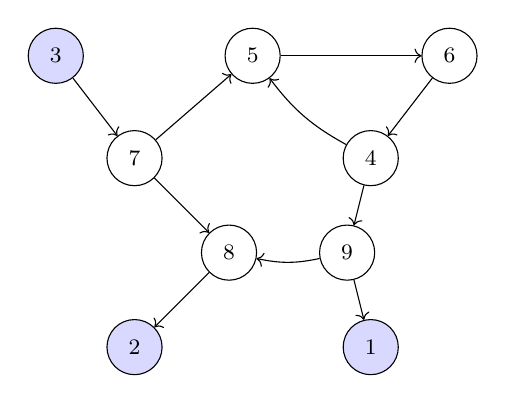
\begin{tikzpicture}[
    node distance=1.6cm,
    every node/.style={circle, draw, minimum size=0.7cm, font=\footnotesize},
    every edge/.style={draw, -Stealth, thick},
    leader/.style={fill=blue!15}
]
\node[leader] (3) at (-2.5, 2.5) {3};
\node (5) at (0, 2.5) {5};
\node (6) at (2.5, 2.5) {6};
\node (7) at (-1.5, 1.2) {7};
\node (4) at (1.5, 1.2) {4};
\node (8) at (-0.3, 0) {8};
\node (9) at (1.2, 0) {9};
\node[leader] (2) at (-1.5, -1.2) {2};
\node[leader] (1) at (1.5, -1.2) {1};
\draw[->] (3) -- (7);
\draw[->] (7) -- (5);
\draw[->] (5) -- (6);
\draw[->] (6) -- (4);
\draw[->] (7) -- (8);
\draw[->] (4) -- (9);
\draw[->] (8) -- (2);
\draw[->] (9) -- (1);
\draw[->] (4) to[bend left=12] (5);
\draw[->] (9) to[bend left=12] (8);
\end{tikzpicture}
\caption{Communication digraph for Example~1 ($N=9$, $\mu=3$). Blue nodes are leaders.}
\label{fig:graph9}
\end{figure}

The model-based DARE solution gives
\begin{equation*}
P^* = \begin{bmatrix} 2.3671 & 1.1180 \\ 1.1180 & 2.5875 \end{bmatrix}, \quad
F = \begin{bmatrix} 2.3016 & 5.4481 \end{bmatrix}, \quad G = 4.2973.
\end{equation*}

\subsubsection{State Feedback Q-Learning Results}

Algorithm~\ref{alg:sf_ql} is applied to a single agent ($l = 3$, $L \geq 6$). Fig.~\ref{fig:sf_conv_ex1} shows convergence in $\sim$18 iterations to machine precision. Table~\ref{tab:reproduction} confirms that the Q-learned gains match the model-based DARE solution from~\cite{cacace2024} to at least 8 significant digits, verifying exact reproduction of the model-based design.

\begin{table}[htbp]
\centering
\caption{Reproduction verification: Q-learned vs.\ model-based gains for Example~1.}
\label{tab:reproduction}
\small
\begin{tabular}{lccc}
\toprule
Quantity & Model-based~\cite{cacace2024} & Q-learned & $\|$Error$\|$ \\
\midrule
$P^*_{11}$ & 2.3671 & 2.3671 & $<10^{-8}$ \\
$P^*_{12}$ & 1.1180 & 1.1180 & $<10^{-8}$ \\
$P^*_{22}$ & 2.5875 & 2.5875 & $<10^{-8}$ \\
$F$ & $[2.3016,\; 5.4481]$ & $[2.3016,\; 5.4481]$ & $<10^{-9}$ \\
$G$ & 4.2973 & 4.2973 & $<10^{-9}$ \\
\bottomrule
\end{tabular}
\end{table}

\begin{figure*}[!htbp]
    \centering
    \includegraphics[width=\textwidth]{figure3_state_convergence_final.png}
    \caption{State feedback Q-learning convergence for Example~1. Left: Bellman error. Center: H-matrix error. Right: gain error.}
    \label{fig:sf_conv_ex1}
\end{figure*}

Fig.~\ref{fig:sf_traj_ex1} shows multi-consensus trajectories using centralized ($\kappa = 2$), distributed ($\kappa = 2$, $\gamma = 2$), and standard ($\kappa = 0.28$~\cite{ma2015}) protocols. Convergence is achieved in $\sim$8, $\sim$12, and $\sim$150 steps respectively. The Q-learned gains produce trajectories indistinguishable from the model-based results in~\cite[Fig.~3]{cacace2024}, confirming that the data-driven approach exactly recovers the DARE solution.

\begin{figure*}[!htbp]
    \centering
    \includegraphics[width=0.85\textwidth]{figure3_state_feedback_final.png}
    \caption{Multi-consensus trajectories with state feedback Q-learned gains for Example~1. Top: consensus error. Rows 2--4: centralized, distributed ($\gamma = 2$), standard protocol.}
    \label{fig:sf_traj_ex1}
\end{figure*}

\subsubsection{Output Feedback Q-Learning Results}

Algorithm~\ref{alg:ofb_ql} uses $y_k = [1 \; 0]x_k$ with dead-beat parameterization ($\tilde{l} = 5$). Fig.~\ref{fig:ofb_conv_ex1} shows convergence in $\sim$25 iterations.

\begin{figure*}[!htbp]
    \centering
    \includegraphics[width=\textwidth]{figure3_output_convergence_final.png}
    \caption{Output feedback Q-learning convergence for Example~1.}
    \label{fig:ofb_conv_ex1}
\end{figure*}

Fig.~\ref{fig:ofb_traj_ex1} confirms that the output feedback gains, deployed via the reconstructed disagreement feedback~\eqref{eq:disagreement}, produce trajectories virtually identical to the state feedback case, validating Proposition~\ref{prop:disagreement}.

\begin{figure*}[!htbp]
    \centering
    \includegraphics[width=\textwidth]{figure3_output_feedback_final.png}
    \caption{Multi-consensus with output feedback Q-learned gains for Example~1. Trajectories are virtually identical to the state feedback case (Fig.~\ref{fig:sf_traj_ex1}), validating Proposition~\ref{prop:disagreement}.}
    \label{fig:ofb_traj_ex1}
\end{figure*}

\FloatBarrier

\subsection{Example 2: Formation Control ($N = 6$, $T = 0.1$~s)}
\label{subsec:sim2}

We consider $N = 6$ continuous-time double integrator agents over the ring digraph in Fig.~\ref{fig:graph6}, which has one reach. Setting $x_i = \col(\zeta_i - \sigma_i, \dot{\zeta}_i)$, the discrete-time model with $T = 0.1$~s uses $Q = 5I_4$, $\kappa = 2$, $\gamma = 33$. The formation is a regular hexagon. This scenario represents a practical UAV coordination problem~\cite{dony2021distributed,dony2021robust}: each agent controls its 2D position and velocity to achieve a desired geometric formation while communicating only with neighbors. The data-driven approach is particularly relevant here because the discrete-time model depends on the sampling period $T$ through the matrix exponential $A = \exp(A_c T)$, and discretization errors are unavoidable in practice.

\begin{figure}[!htb]
\centering
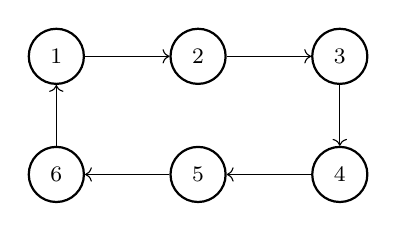
\begin{tikzpicture}[
    node distance=1.8cm,
    every node/.style={circle, draw, minimum size=0.7cm, font=\footnotesize, thick},
    every edge/.style={draw, -Stealth, thick}
]
\node (1) at (0, 1.5) {1};
\node (2) at (1.8, 1.5) {2};
\node (3) at (3.6, 1.5) {3};
\node (6) at (0, 0) {6};
\node (5) at (1.8, 0) {5};
\node (4) at (3.6, 0) {4};
\draw[->] (1) -- (2);
\draw[->] (2) -- (3);
\draw[->] (3) -- (4);
\draw[->] (4) -- (5);
\draw[->] (5) -- (6);
\draw[->] (6) -- (1);
\end{tikzpicture}
\caption{Ring digraph for Examples~2 and~3 ($N=6$, $\mu=1$).}
\label{fig:graph6}
\end{figure}

\subsubsection{State Feedback Results}

With $l = 6$, $L \geq 21$, Fig.~\ref{fig:sf_conv_ex2} shows convergence in $\sim$130 iterations. Fig.~\ref{fig:sf_traj_ex2} shows agents converging to the hexagonal formation.

\begin{figure*}[!htbp]
    \centering
    \includegraphics[width=\textwidth]{figure5_state_convergence_final.png}
    \caption{State feedback Q-learning convergence for Example~2 ($T = 0.1$~s).}
    \label{fig:sf_conv_ex2}
\end{figure*}

\begin{figure*}[!htbp]
    \centering
    \includegraphics[width=\textwidth]{figure5_state_feedback_final.png}
    \caption{Formation control with state feedback Q-learned gains for Example~2 ($T = 0.1$~s). Agents converge to hexagonal formation within 6~s.}
    \label{fig:sf_traj_ex2}
\end{figure*}

\subsubsection{Output Feedback Results}
With $\tilde{l} = 14$, output feedback Q-learning converges in $\sim$250 iterations with $\|G - G^*\| < 10^{-7}$. The resulting formation trajectories, deployed via~\eqref{eq:disagreement}, are virtually identical to the state feedback case in Fig.~\ref{fig:sf_traj_ex2}, consistent with Proposition~\ref{prop:disagreement}. Trajectory figures are omitted as they visually coincide with the state feedback results.

\FloatBarrier

\subsection{Example 3: Formation Control ($N = 6$, $T = 1.0$~s)}
\label{subsec:sim3}

The same setup as Example~2 with $T = 1.0$~s and $\gamma = 28$.

\subsubsection{State Feedback Results}

Fig.~\ref{fig:sf_conv_ex3} shows convergence in only $\sim$15 iterations---the fastest among all examples due to better conditioning at the larger sampling period. Fig.~\ref{fig:sf_traj_ex3} shows the formation trajectories.

\begin{figure*}[!htbp]
    \centering
    \includegraphics[width=\textwidth]{figure6_state_convergence_final.png}
    \caption{State feedback convergence for Example~3 ($T = 1.0$~s). Convergence in $\sim$15 iterations.}
    \label{fig:sf_conv_ex3}
\end{figure*}

\begin{figure*}[!htbp]
    \centering
    \includegraphics[width=\textwidth]{figure6_state_feedback_final.png}
    \caption{Formation control with state feedback Q-learned gains for Example~3 ($T = 1.0$~s). Faster convergence than Example~2 due to better DARE conditioning.}
    \label{fig:sf_traj_ex3}
\end{figure*}

\subsubsection{Output Feedback Results}
Output feedback Q-learning converges in $\sim$25 iterations with $\|G - G^*\| < 10^{-8}$, and the formation trajectories match the state feedback case. Trajectory figures are omitted as they visually coincide with the state feedback results.

\FloatBarrier

\subsection{Robustness to Parametric Uncertainty}
\label{subsec:robustness}

Because the Bellman equations~\eqref{eq:bellman_consensus} and~\eqref{eq:ofb_bellman} are built entirely from measured data, the Q-learned gains are matched to the true plant from which the data is collected. To quantify this advantage under model uncertainty, we consider Example~1 with a perturbed system matrix $A_{\mathrm{true}} = A_{\mathrm{nom}} + \Delta A$, where $\Delta A = \delta \begin{bsmallmatrix} 0 & 1 \\ 0 & 0 \end{bsmallmatrix}$ represents uncertainty in the $(1,2)$ entry of the double integrator. The model-based approach computes gains from the nominal $A_{\mathrm{nom}}$ via the DARE, while Q-learning extracts gains from data collected on the true (perturbed) system.

Fig.~\ref{fig:robustness} presents four analyses. Panel~(a) shows that, in this example, the maximum closed-loop spectral radius $\max_k \rho(\bar{A}_k)$ for the model-based gains increases monotonically with the perturbation magnitude, approaching the stability boundary $\rho = 1$, while the Q-learned spectral radius remains smaller over the tested perturbation range. At $\delta = 1.0$, the model-based margin is $1 - 0.76 = 0.24$ versus $1 - 0.25 = 0.75$ for Q-learning---a threefold improvement. Panel~(b) shows that the relative LQR cost penalty of model-based gains grows to 37\% at $\delta = 1.0$. Panel~(c) shows the velocity trajectories at $\delta = 0.3$: the Q-learned gains (dashed) achieve tighter consensus than the model-based gains (solid), consistent with the spectral radius difference. Panel~(d) compares the gain values at $\delta = 0.5$: the Q-learned gains match the true DARE solution to machine precision, while the nominal model gains deviate significantly.

\begin{figure*}[!htbp]
    \centering
    \includegraphics[width=0.9\textwidth]{robustness_simulation.png}
    \caption{Robustness analysis under parametric uncertainty $\Delta A_{12}$. Top-left: stability margin. Top-right: cost penalty. Bottom-left: velocity trajectories at $\delta = 0.3$ (solid = model-based, dashed = Q-learned). Bottom-right: gain comparison at $\delta = 0.5$.}
    \label{fig:robustness}
\end{figure*}

\FloatBarrier

\subsection{Example 4: Vehicle Platoon with Aerodynamic Drag}
\label{subsec:sim4}

To demonstrate the practicality of the proposed framework, we consider a vehicle platoon control problem---a representative application in intelligent transportation systems. A string of $N = 5$ vehicles with aerodynamic drag must achieve velocity consensus while maintaining a desired inter-vehicle spacing of $d_{\mathrm{ref}} = 10$~m. Each vehicle has the discrete-time dynamics
\begin{equation}
A = \begin{bmatrix} 1 & T \\ 0 & 1 - bT \end{bmatrix}, \quad B = \begin{bmatrix} T^2/2 \\ T \end{bmatrix},
\end{equation}
where $T = 0.1$~s is the sampling period and $b = 0.1$~s$^{-1}$ is the drag coefficient. Unlike the double integrator, this system includes velocity-dependent dissipation ($bT = 0.01$), making it a more realistic model of longitudinal vehicle dynamics. The state is $x_i = [\zeta_i - d_{\mathrm{ref}}\cdot i, \; \dot{\zeta}_i]^\top$ (spacing error and velocity), and the communication graph is a directed string $1 \to 2 \to 3 \to 4 \to 5$.

Algorithm~\ref{alg:sf_ql} converges in $\sim$106 iterations with $\|F - F^*\| < 10^{-9}$. Fig.~\ref{fig:platoon} shows the platoon behavior under Q-learned consensus gains: vehicles achieve the desired 10~m spacing with velocity consensus within $\sim$5~s, and control inputs remain smooth and bounded. The data-driven approach is particularly advantageous here because the drag coefficient $b$ may vary with speed and environmental conditions, making the exact discrete-time model uncertain.

For the output feedback case, using $C = [1 \;\; 0]$ (position-only measurement), Algorithm~\ref{alg:ofb_ql} converges in $\sim$140 iterations and deploys the reconstructed disagreement feedback~\eqref{eq:disagreement}, confirming that the platoon can be controlled using only position sensors without velocity measurement.

\begin{figure*}[!htbp]
    \centering
    \includegraphics[width=\textwidth]{platoon_trajectories.png}
    \caption{Vehicle platoon control with Q-learned gains ($N=5$, $b=0.1$~s$^{-1}$, $T=0.1$~s). Left to right: positions, velocities, spacing errors, control inputs.}
    \label{fig:platoon}
\end{figure*}

\FloatBarrier

\subsection{Summary of Results}
\label{subsec:sim_summary}

Table~\ref{tab:summary} summarizes convergence across all examples.

\begin{table}[htbp]
\centering
\caption{Summary of Q-learning convergence across examples.}
\label{tab:summary}
\small
\begin{tabular}{lccccc}
\toprule
Example & $n$ & $m$ & Method & Iterations & $\|K - K^*\|$ \\
\midrule
1 ($N{=}9$, $\mu{=}3$) & 2 & 1 & State FB & 18 & $10^{-9}$ \\
& & & Output FB & 25 & $\|G - G^*\| < 10^{-8}$ \\
\midrule
2 ($T{=}0.1$s) & 4 & 2 & State FB & 130 & $10^{-8}$ \\
& & & Output FB & 250 & $\|G - G^*\| < 10^{-7}$ \\
\midrule
3 ($T{=}1.0$s) & 4 & 2 & State FB & 15 & $10^{-10}$ \\
& & & Output FB & 25 & $\|G - G^*\| < 10^{-8}$ \\
\midrule
4 (Platoon) & 2 & 1 & State FB & 106 & $10^{-9}$ \\
& & & Output FB & 140 & $\|G - G^*\| < 10^{-8}$ \\
\bottomrule
\end{tabular}
\end{table}

\FloatBarrier

%% ===================================================================
\section{Discussion}
\label{sec:discussion}
%% ===================================================================

This section interprets the results and analyzes the practical properties of the proposed framework: computational cost, scalability with network size, selection of the distributed iteration depth, communication requirements, the nature of the observed robustness advantage, and limitations.

\subsection{Computational Complexity}
\label{subsec:complexity}

Each iteration of Algorithm~\ref{alg:sf_ql} requires solving an $l(l+1)/2$-dimensional least-squares problem, with computational cost $\mathcal{O}(L \cdot l^2 + l^6)$ per iteration and total cost $\mathcal{O}(J \cdot l^6)$, where $J$ is the number of iterations to convergence and $l = n+m$. For comparison, the model-based DARE is solved via the Schur decomposition in $\mathcal{O}(n^3)$. While Q-learning is more expensive per solve, it avoids the cost and error of system identification, which can be substantial for high-dimensional or poorly conditioned systems. The output-feedback algorithm has the same structure with $\tilde{l} = mn+pn+m$ in place of $l$; the larger regression dimension explains the slower convergence observed in Table~\ref{tab:summary} (e.g., 250 vs.\ 130 iterations in Example~2).

\subsection{Scalability with Network Size}
\label{subsec:scalability}

A key practical property, confirmed across all examples, is that the learning cost is \emph{independent} of the network size $N$. Since the DARE depends only on $(A,B,Q)$ and not on the communication graph, Algorithms~\ref{alg:sf_ql}--\ref{alg:ofb_ql} are executed once on a single agent, and the learned gains are deployed across all $N$ agents with their respective coupling gains $\kappa_i$. Whether the network contains 5 or 500 agents, the learning phase is identical. This contrasts with distributed RL methods such as~\cite{zhang2011}, where each agent must learn concurrently and the learning cost scales with $N$.

\subsection{Model-Free Selection of the Distributed Iteration Depth $\gamma$}
\label{subsec:gamma}

The minimum number of distributed consensus steps $\gamma_{\min}$ from~\cite[Thm.~3.4]{cacace2024} depends on $\rho(G)$ and $\rho(A - BK^*)$. The spectral radius $\rho(G) = \rho(H_{uu}^* - I_m)$ is directly available from the converged H-matrix without any model knowledge. Quantities involving the closed-loop matrix $A - BK^*$, however, are not directly available from $H^*$ alone. In a fully data-driven implementation, one may collect closed-loop data under the converged policy $K^*$ and estimate
\begin{equation}
\hat{A}_{\mathrm{cl}} = X^+ X^\dagger,
\label{eq:Acl}
\end{equation}
where $X = [x_0, \ldots, x_{T-1}]$, $X^+ = [x_1, \ldots, x_T]$, and $X^\dagger$ denotes the pseudoinverse; then $\rho(A - BK^*)$ is approximated by $\rho(\hat{A}_{\mathrm{cl}})$. Alternatively, $\gamma$ can be selected empirically by increasing the number of inner consensus iterations until the distributed input $v_i(t,\gamma)$ is sufficiently close to the centralized input~\eqref{eq:u_central}, which is the procedure used in Examples~2 and~3 ($\gamma = 33$ and $\gamma = 28$, respectively).

\subsection{Communication Requirements}
\label{subsec:communication}

The distributed $\gamma$-step algorithm~\eqref{eq:dist_init}--\eqref{eq:dist_iter} requires $\gamma$ communication rounds per sampling period $T$, introducing a trade-off: larger $\gamma$ improves the approximation of the centralized solution~\eqref{eq:u_central} but increases the communication burden. In practice, communication latency constrains $\gamma \leq T / \tau_{\mathrm{comm}}$, where $\tau_{\mathrm{comm}}$ is the per-round communication delay. Combining the predictor-based protocol with event-triggered communication strategies is a promising direction to reduce this overhead while preserving consensus guarantees. Note that this requirement is inherited from the protocol of~\cite{cacace2024} and is not introduced by the learning layer: once learned, the gains impose no additional communication.

\subsection{Interpretation of the Robustness Results}
\label{subsec:robust_disc}

The robustness study of Section~\ref{subsec:robustness} demonstrates \emph{exactness on the true plant}: when data is drawn from the true (perturbed) system, Q-learning recovers the DARE solution of that system to machine precision, whereas the model-based design remains anchored to the nominal model and its stability margin erodes as the perturbation grows. We emphasize that this is a property of data-driven exactness rather than a formal robustness margin; the observed threefold margin improvement at $\delta = 1.0$ and the 37\% cost penalty of the nominal design quantify the practical consequence of this distinction in the example considered. The insight transfers directly to applications such as the vehicle platoon of Section~\ref{subsec:sim4}, where physical parameters (e.g., the drag coefficient) vary with operating conditions and an exact nominal model is unavailable.

\subsection{Limitations}
\label{subsec:limitations}

Three limitations delineate the scope of the present results. First, the framework assumes identical linear agents; heterogeneous or nonlinear dynamics would break the single-agent learning architecture and the quadratic Q-function structure, respectively. Second, the convergence guarantees assume noise-free state or output \emph{measurements}; exploration noise in the input is provably bias-free (Theorems~\ref{thm:sf_convergence} and~\ref{thm:ofb_convergence}), but measurement noise would require an instrumental-variable or total-least-squares treatment. Third, the excitation (rank) condition on the regression matrix must be verified in practice, which constrains the choice of probing signals during the learning phase.

%% ===================================================================
\section{Conclusions}
\label{sec:conc}
%% ===================================================================

This paper presented data-driven Q-learning algorithms for learning the gains of a predictor-based consensus protocol for discrete-time linear MAS. By exploiting the DARE--LQR structural equivalence, the state feedback algorithm extracts both consensus gains from single-agent data, and the output feedback extension---building on the input-output Q-learning of~\cite{rizvi2022}---reconstructs the inter-agent disagreement feedback required by the protocol rather than the absolute regulator. The learned gains exactly satisfy the DARE, so all consensus and multi-consensus guarantees of~\cite{cacace2024}, including arbitrary convergence rate, are inherited; this exactness was validated numerically to machine precision against the model-based benchmark, and the robustness study showed superior stability margins under parametric uncertainty, with a vehicle platoon example confirming practical applicability. The novelty of the work lies in the linkage between data-driven LQR reinforcement learning and predictor-based discrete-time consensus---two established areas not previously connected---and its impact is to extend a consensus design with arbitrary convergence rate to settings where the agent model is unknown.

Future directions include heterogeneous MAS (requiring distributed Q-learning), time-varying topologies with event-triggered communication, nonlinear extensions via Koopman lifting~\cite{dony2024koopman}, and safety enforcement through control barrier functions~\cite{dony2025debf}.

%% ===================================================================
\section*{Declaration of Competing Interest}
%% ===================================================================

The authors declare that they have no known competing financial interests or personal relationships that could have appeared to influence the work reported in this paper.

%% ===================================================================
\section*{Funding}
%% ===================================================================

This research did not receive any specific grant from funding agencies in the public, commercial, or not-for-profit sectors.

%% ===================================================================
\section*{Data Availability}
%% ===================================================================

The simulation scripts that support the findings of this study are available from the corresponding author upon reasonable request.

%% ===================================================================
\section*{CRediT Authorship Contribution Statement}
%% ===================================================================

\textbf{Md Nur-A-Adam Dony:} Conceptualization, Methodology, Software, Formal analysis, Investigation, Validation, Writing -- original draft, Visualization.
\textbf{Syed Ali Asad Rizvi:} Conceptualization, Methodology, Supervision, Writing -- review \& editing.

%% ===================================================================
%% References (numbered in order of first appearance)
%% ===================================================================
\begin{thebibliography}{99}

\bibitem{francis2016}
B.A. Francis, M. Maggiore, Flocking and Rendezvous in Distributed Robotics, Springer, 2016.

\bibitem{dony2021distributed}
M.N.A. Dony, W. Dong, Distributed robust formation flying and attitude synchronization of spacecraft, J. Aerosp. Eng. 34 (2021) 04021002.

\bibitem{dong2020tracking}
W. Dong, M.N.A. Dony, M. Rafat, Tracking control of vertical taking-off and landing vehicles with parametric uncertainty, Int. J. Adapt. Control Signal Process. 34 (2020) 1600--1612.

\bibitem{dorfler2014}
F. D\"{o}rfler, F. Bullo, Synchronization in complex networks of phase oscillators: A survey, Automatica 50 (6) (2014) 1539--1564.

\bibitem{li2010}
Z. Li, Z. Duan, G. Chen, L. Huang, Consensus of multiagent systems and synchronization of complex networks: A unified viewpoint, IEEE Trans. Circuits Syst. I Reg. Papers 57 (1) (2010) 213--224.

\bibitem{battistelli2014}
G. Battistelli, L. Chisci, G. Mugnai, A. Farina, A. Graziano, Consensus-based linear and nonlinear filtering, IEEE Trans. Autom. Control 60 (5) (2015) 1410--1415.

\bibitem{proskurnikov2017}
A.V. Proskurnikov, R. Tempo, A tutorial on modeling and analysis of dynamic social networks. Part I, Annu. Rev. Control 43 (2017) 65--79.

\bibitem{li2014}
Z. Li, G. Wen, Z. Duan, W. Ren, Designing fully distributed consensus protocols for linear multi-agent systems with directed graphs, IEEE Trans. Autom. Control 60 (4) (2015) 1152--1157.

\bibitem{liu2021}
Z. Liu, A. Saberi, A.A. Stoorvogel, D. Nojavanzadeh, Scale-free collaborative protocol design for synchronization of multi-agent systems with arbitrary fast convergence, J. Franklin Inst. 358 (9) (2021) 4864--4882.

\bibitem{ma2015}
Q. Ma, F.L. Lewis, S. Xu, Cooperative containment of discrete-time linear multi-agent systems, Int. J. Robust Nonlinear Control 25 (7) (2015) 1007--1018.

\bibitem{ren2010}
W. Ren, Y. Cao, Distributed Coordination of Multi-Agent Networks, Springer, 2010.

\bibitem{xiao2004}
L. Xiao, S. Boyd, Fast linear iterations for distributed averaging, Syst. Control Lett. 53 (1) (2004) 65--78.

\bibitem{cacace2024}
F. Cacace, M. Mattioni, S. Monaco, D. Normand-Cyrot, Consensus and multi-consensus for discrete-time LTI systems, Automatica 166 (2024) 111718.

\bibitem{monaco2019}
S. Monaco, L. Ricciardi~Celsi, On multi-consensus and almost equitable graph partitions, Automatica 103 (2019) 53--61.

\bibitem{dony2020tracking}
M.N.A. Dony, M. Rafat, W. Dong, Distributed command filtered robust tracking control of wave-adaptive modular vessel with uncertainty, in: Proc. 2020 American Control Conference (ACC), Denver, CO, 2020, pp. 2118--2123.

\bibitem{dony2021robust}
M.N.A. Dony, Robust Distributed Formation Control of UAVs with Higher-Order Dynamics, Master's thesis, The University of Texas Rio Grande Valley, 2021.

\bibitem{lewis2009}
F.L. Lewis, D. Vrabie, Reinforcement learning and adaptive dynamic programming for feedback control, IEEE Circuits Syst. Mag. 9 (3) (2009) 32--50.

\bibitem{bradtke1994}
S.J. Bradtke, B.E. Ydstie, A.G. Barto, Adaptive linear quadratic control using policy iteration, in: Proc. American Control Conference, 1994, pp. 3475--3479.

\bibitem{rizvi2022}
S.A.A. Rizvi, Z. Lin, Output Feedback Reinforcement Learning Control for Linear Systems, Control Engineering Series, Springer Nature, 2022.

\bibitem{zhang2011}
H. Zhang, F.L. Lewis, A. Das, Optimal design for synchronization of cooperative systems: State feedback, observer and output feedback, IEEE Trans. Autom. Control 56 (8) (2011) 1948--1952.

\bibitem{dony2025debf}
M.N.A. Dony, M.E. Khallil, Adaptive reinforcement learning with control barrier functions for safe state avoidance in discrete event systems, in: Proc. 8th IEOM Bangladesh Int. Conf., Dhaka, Bangladesh, 2025.

\bibitem{dony2026battery}
M.N.A. Dony, B. Arhin, Data-driven distributed battery state-of-charge balancing using neural network-based open circuit voltage learning, IFAC J. Syst. Control 36 (2026) 100415.

\bibitem{dony2024koopman}
M.N.A. Dony, Integrating Koopman theory and Lyapunov stability for enhanced model predictive control in nonlinear systems, ResearchGate preprint, 2024. https://doi.org/10.13140/RG.2.2.17950.31046.

\bibitem{caughman2006}
J.S. Caughman, J.J.P. Veerman, Kernels of directed graph Laplacians, Electron. J. Combin. 13 (1) (2006) 39.

\bibitem{hewer1971}
G.A. Hewer, An iterative technique for the computation of the steady state gains for the discrete optimal regulator, IEEE Trans. Autom. Control 16 (4) (1971) 382--384.

\end{thebibliography}

\end{document}
